% \begin{figure}[htb]	
% \center%6.3
% 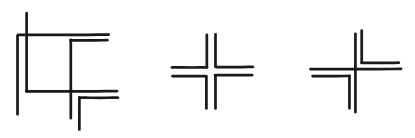
\includegraphics[width=10cm]{./img/representacaociclotam4.png}
% \caption{$B_{1}$-EPG representation of the induced cicle of size 4: frame (in left), true pie (center) and false pie (in right), \cite{golumbic2009}.}

% \end{figure}

\begin{figure}[htb]
  \centering
%segundo bloco de figuras
  \begin{tabular}{c c c c c }
    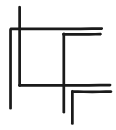
\includegraphics[width=2.3cm]{./img/representacaociclotam41.png}  
    & &
\includegraphics[width=2.5cm]{./img/representacaociclotam42.png} 
    & &
 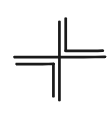
\includegraphics[width=2.5cm]{./img/representacaociclotam43.png} \\%[\abovecaptionskip]
    {\footnotesize (a) Frame}  & &  {\footnotesize (b) True pie} & & {\footnotesize (c) False pie} %\label{fig:frame}
  \end{tabular}
  \caption{$B_{1}$-EPG representation of the induced cycle of size 4}\label{fig:ciclotam4}
\end{figure} 